\documentclass[12pt]{report}
\usepackage{graphicx}
\usepackage{indentfirst}
\usepackage{url}
\usepackage{apacite}
\bibliographystyle{apacite}


\title{Classification of Ailments Given Description of Symptoms}
\author{Urmzd Mukhammadnaim \\ Ben MacDonald}
\graphicspath{{./images/}}

\begin{document}
\maketitle
\tableofcontents
\begin{abstract}
	In this paper, we address the challenges experienced in the preliminary research phase
	of ailment diagnosis performed by many individuals prior to visiting a
	healthcare professional. Due to the large quantity of varying results appearing
	once someone searches their current symptoms, we developed a convolutional
	neural network (CNN) that reduces this clutter by returning only the most
	probable medical condition given the user's description.
	To address the problem, we introduce two CNN implementations with different
	preprocessors. The first implementation explores the use of a One Hot Encoder,
	while the second implementation utilizes a FastText model trained via
	unsupervised learning. Through the retrieval of open source data from various medical platforms such
	as UpToDate and Mayo Clinic, a recall value of 90\% is achieved.
\end{abstract}

\chapter{Introduction}
Individuals are able to obtain data in a wide array of topics nearly
instantaneously through the internet. Among these searches are descriptions of
symptoms people are experiencing in an attempt to find the primary cause.
According to a study conducted by Eligibility, approximately 89\% of American
patients search what they are experiencing on a search engine prior to visiting
their doctor \cite{guarino_2019}.

The result of the query often results in a list of websites such as WebMD and
MayoClinic. These pages will typically contain an ailment, a description,
a list of potential symptoms, as well as possible treatments. In these
encounters, the user may have a negative experience as a direct result of
the overwhelming quantity of information potentially shown. Additionally,
based on the description provided, the user may also find conflicting resources.
Contradictory information is further exaggerated by broader descriptions,
such as "pounding head", which can be attributed to a large number of illnesses.

This problem led us to consider how to structure a process that streamlines this
preliminary research. As opposed to using a search engine which indexes its data primarly
on a platform's metadata, we viewed the ideal scenario as condensing the actions
to entering the text into a model that would provide the singular most probable
diagnosis. To implement this functionality, we determined three necessary
objectives:

\begin{itemize}
	\item Acquire a dataset that includes the descriptions of an ailment.
	\item Construct a model that produces a probability distribution of all the available classifications.
	\item Utilize the developed model to classify symptom descriptions as an ailment.
\end{itemize}

To develop our dataset, we scraped text from websites which included
descriptions of ailments and their associated symptoms. Moreover, only websites
containing "semi-informal" terminology was used. This was done in order to
improve the similarity between the training data and the input the model would
likely recieve from a user. There were several possible approaches we could have
taken to develop a model for this multi-classification problem.
Among these, we found that CNNs
provided a flexible model which performed well with classifying text, and has been
used to classify symptoms at a sentence level to a great degree
of success\cite{HughesLKS17}. Afterwards, we were able to observe the network's capacity to classify
the dataset, and proceeded to test its ability to categorize our
own descriptions of the three ailments, depression, migraines and tetanus.

\chapter{Related Works}
There are various ways in which we could have the user interact with the
model. Kurup and Shetty document their creation of an conversational chatbot
that utilizes neural networks and Decision Tree Classifiers to classify the
ailment that a particular user is experiencing given responses to a
questionnaire. Due to a sparsity of publicly available
datasets, they created a file with custom patterns classified by their
expected responses. They then used this to train a neural network composed of two
fully-connected layers, as well as dropout layers to prevent overfitting. The Decision
Tree Classifier was then trained with a dataset of binary values indicating
whether a symptom is associated with a particular ailment. When
interacting with the neural network via messaging, the user could indicate
that they wished to take a “prognosis quiz”, where they would answer yes or
no to experiencing a symptom. The neural network was able to achieve
an accuracy of 95\%. The Decision Tree Classifier functioned as intended. The
implementation, however, does not provide a seamless series of interactions
for the user as they converse with the chatbot\cite{kurup_2021}.

Utilizing CNNs in Natural Language Processing (NLP) is growing in popularity,
with several papers documenting their efficacy in text classification. Hughes
et al describe their use of a Word2vec model and CNN to classify medical text
at the sentence level, and compared their accuracy to other NLP techniques.
Their vectorization model was trained through the use of a dataset containing
15,000 clinical research documents. A series of clinical articles were
labeled as one of 26 medical categories with 4000 sentences being
randomly selected for each classification. These sentences were then vectorized
by the Word2vec model and used to train the CNN. The setup went on to
perform with an accuracy of 68\%. The model outperformed other text classification techniques
such as logistic regression using bag-of-words, which possessed an
accuracy of 51\%. The former model was effective at displaying the success of CNNs
in this context and on a larger scale with 26 individual ailments. The use of
word embeddings provided the neural network greater possible depths of
understanding for the relationships between separate words and their
associations. These benefits, however, are dependent on the large quantity of
available data to train the Word2vec model\cite{HughesLKS17}.

There is a clear distinction between classifying professional medical text
and casual descriptions with informal terminology. Gambhir et al studied the
accuracy of a convolutional neural network-long short term memory (CNN-LSTM)
model in the context of monitoring social media for posts mentioning a drug name.
It would classify them as one of three categories indicating the degree of medication.
The CNN-LSTM performed with the greatest precision in
comparison to other tested models, but a lower recall than the LSTM model.
The distinction between professional medical text and casual descriptions is
an important one to make. There is a large difference between the two in
terms of sentence structure and diction. Professional text can contain a
variety of rare terms which can impact a model's
capacity to properly classify a description, should a large corpus be
unavailable\cite{tokala-etal-2018-deep}.


\chapter{Methodology}
\section{Data Collection}
One of the challenges in this endeavour was finding accessible and well
documented open-source records. As medical data was difficult to come across, due
to HIPAA, PIPEDA, and other laws that bar hospitals, and various medical
organizations from distributing patients' health documents, we had to settle
for medical encyclopedias and articles. To ensure a baseline consistency in the data used across
the desired classifications, the descriptions were pulled from the same sites.
Between articles on the same website, however, the detail in which the article
was written varied greatly. Some articles had more advertisements, others had
more embedded miscellaneous content, and most of them differed in document
structure. In other words, the data could not be accessed directly via its url
and Document Object Model (DOM) selector. The data was collected using the top-most DOM element
encapsulating all the desired information, resulting in documents with
irrelevant content within them.  As a result, a greater burden was moved onto
the preprocessor to ensure clean and usable data was entering the CNN. It
should also be noted that we used the automation library “pyppeteer” in lieu of
a simple “GET” retrieval of the HTML document to prevent issues accessing the
data due to Server Side Rendering (SSR). As a result, there was greater
overhead during this phase.

\section{Data Processing}
After the extraction and consequent concatenation of the documents for each
classification, we explored two preprocessor implementations. We first describe
the use of One Hot Encoder\cite{scikit-learn} and Witten-Bell Probability Distribution\cite{bird2009natural}, to retain
morphological-level information and generate unique sets of words that could
later be fed into the CNN. Subsequently, we analyze the use of the FastText\cite{rehurek2011gensim}
model as a means of retaining semantic-level information, and ensuring words
with similar words appear closer together in the subspace.

\subsection{One Hot Encoding and Witten Bell Generation}
After the documents were tokenized, the text was piped into the transformer $T_1$ which applied a
series of reduction operations to remove punctuation, ultimately breaking the words
into their stems. The result of $T_1$ consisted of a set of unique stems $D_n$,
where $n$ represents the order in which the document was processed.
After $T_1$ was applied to all documents, the union of all the sets was taken to
form the vocabulary $V$. Subsequently, $V$ was fed into the \emph{FreqDist} class from
the \emph{nltk.probability} package to allow the subsequent usage of the
\emph{WittenBellProbDist}. By allocating $|V|$ bins, and using the
\emph{FreqDist} of $D_n$, we ended up with an instance of the
\emph{WittenBellProbDist}\cite{bird2009natural} capable of generating ${}_{V}C_{S}$ unique sets,
where $S$ represents the cardinality of the generated set. The described method
was used to prevent clustering of the same words, and ultimately prevent the
model from developing an aptitude for classifing an input based on the
frequency of its instances, instead of the existence of an instance.


After $N$ samples were generated via the \emph{WittenBellProbDist} method\cite{bird2009natural}
described above, we transformed the data using an instance of the
\emph{OneHotencoder}\cite{scikit-learn} class fit on the the vocabulary $V$.
As a result, each word in $D$ had its own unique binary vector, and out-of-vocabulary (OOV)
words were treated as the $0$ vector with size $|V|$.

\subsection{FastText Model}
In the alternative preprocessor, we used the FastText model. Unlike the former method,
no data generation was done. Instead, all documents were tokenized by sentence using
an instance of the \emph{PunktSentenceTokenizer}\cite{bird2009natural}. The sentences were then appended to
a singular file, which served as the corpus for the FastText model. Using an implementation of
the FastText model by \emph{gensim}\cite{rehurek2011gensim}, we trained an unsupervised word embeddings model
capable of translating words into a $R$ dimension vector.
After the FastText model was trained, each word in the vocublary was projected onto
the embedding space, resulting in vectors of cardinality $R$.

While each word had the same length, the sentence length varied. As a result,
a transformer $T_2$ was created to pad the given sequences. The algorithm
applied consisted of retrieving the vector that resulted of a coordinate-wise
max or min. Alternating between max and min operations, we injected the sequence
with the resulting vector from the operating described\cite{2016}.

\section{Training \& Achitecture}
As there existed little data, only 20\% of the input was withheld for validation.
In this section, we describe the reasoning for the architecture we decided upon.
It should be noted that the architecture did not depend on the pre-processor.
Hence, there is no difference in the architecture of the classifier between the two implementations.

\subsection{Layers}
The primary components of the CNN consisted of 2D Convolution layers,
Max Pooling layers, a Flatten layer, Dense layers, Dropout layers and finally a Dense output layer.
The convolution layers were used as a means of determining the dimensions
responsible in classfying an ailment, while the max pooling layers were used to drop
dimensions with little information. After the final pooling layer, the output was passed through a
Flatten layer to reduce the resulting feature map onto a single column matrix, allowing it to be
transformed in later operations.
Afterwards, the resulting output was then passed to a series of alternating
Dense and Dropout layers. The Dense layers were added to ensure
that the CNN would be able to fine tune its mechanisms, likely finding small details in the activation map provided
and over time, make better classifications. The Dropout layers were used to prevent overfitting
as a result of the small dataset. Finally, the last Dense layer was used to reduce
the learned values onto a probability distribution matching the cardinality of the classification size\cite{chollet2015keras}.

\begin{figure}[h!]
	\centering
	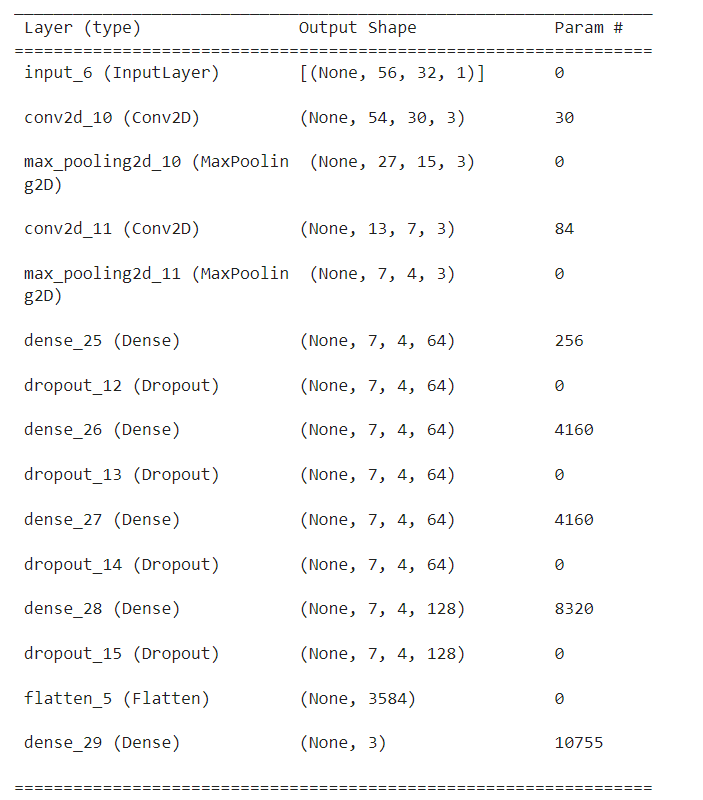
\includegraphics[ width=0.5\textwidth ]{fast-text-summary.png}
	\caption{Fast Text Model Preprocessor - CNN}
\end{figure}

\begin{figure}[h!]
	\centering
	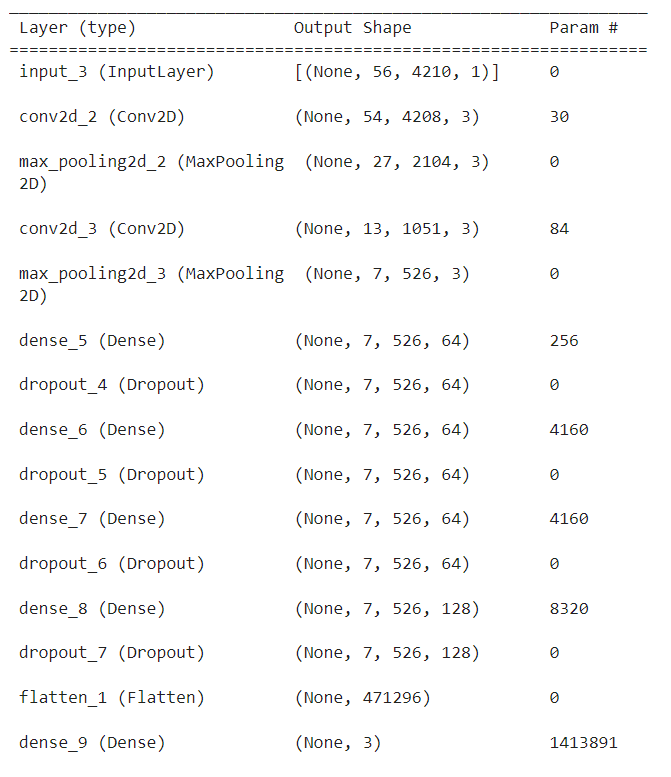
\includegraphics[ width=0.5\textwidth]{one-hot-encoder-summary.png}
	\caption{One Hot Encoding Preprocessor - CNN}
\end{figure}

\section{First Implementation}


\subsection{Results}

\begin{figure}[h!]
	\centering
	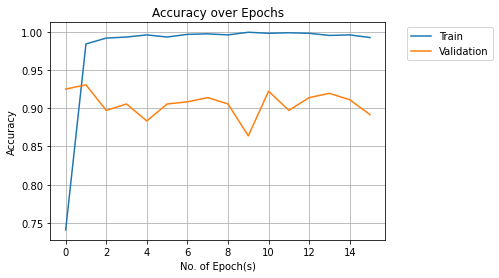
\includegraphics[width=0.5\textwidth]{accuracy.png}
	\caption{One Hot Encoding Preprocessor - CNN Accuracy}
	\label{fig:ohep-acc}
\end{figure}

\begin{figure}[h!]
	\centering
	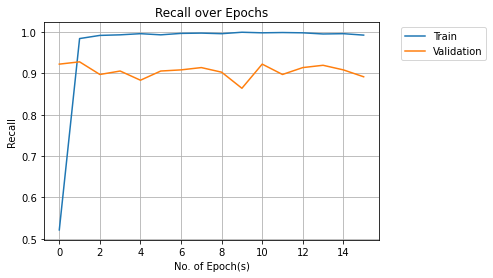
\includegraphics[width=0.5\textwidth]{recall.png}
	\caption{One Hot Encoding Preprocessor - CNN Recall}
	\label{fig:ohep-rec}
\end{figure}

\begin{figure}[h!]
	\centering
	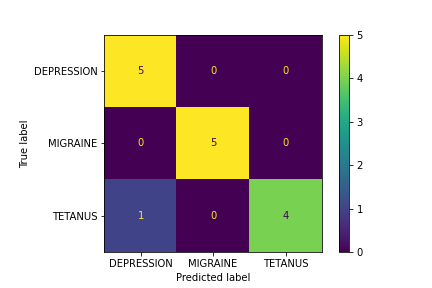
\includegraphics[width=0.5\textwidth]{confusion_matrix_ohe.png}
	\caption{One Hot Encoding Preprocessor - CNN Confusion Matrix}
	\label{fig:ohep-con}
\end{figure}

When observing the accuracy over the number of epochs in the first implementation,
we found that at the first epoch, validation accuracy was higher than training
accuracy with values of 0.925 and 0.74 respectively. For the second epoch and onwards,
however, training accuracy varied around 0.99 and validation accuracy hovered around
0.9. \ref{fig:ohep-acc} and \ref{fig:ohep-rec}, however, are measures of how well the model performed
in regards to classifying the randomized training data. In \ref{fig:ohep-con}, we mapped the
model's capacity to classify our written descriptions as either depression, a
migraine or tetanus.

As observed in \ref{fig:ohep-con}, the model was highly effective at classing descriptions of
depression, migraines and tetanus. Depression possessed a precision of 0.83 and a
recall of 1.0 while tetanus had a precision and recall of 1 and 0.8 respectively.
For migraines, however, the model returned a precision and recall both of 1.

\subsection{Discussion}
There are several factors that play into the model's ability to label these descriptions
accurately. It is evident that the neural network was capable of recognizing the particular
types of words commonly used when describing the three illnesses as scraped from medical
websites. An example of an accurately labelled symptom description tested was "my head
feels like it's spinning, pain in head, pounding throbbing". Keywords that the model
may have recognized in this specific instance were “head”, “spinning”, “pounding” and
“throbbing”. The 750 generated instances for each label used to train the model appear to
have provided a generalized representation of the language used to describe symptoms to make
the model perform with a high level of precision and recall.

The use of One Hot Encoding certainly impacted the run-time performance of the model.
Since every single column represented a unique word, the dimensions of the sentence matrix
were 56x4210. This was a result of the 4210 unique stems of words in the corpus. This large
number of features slowed the model dramatically, and led to the epoch training time to increase.
In an attempt to reduce dimensionality and provide the model with some form of semantic
meaning, we deecided to use word embeddings in the next implementation.

\section{Second Implementation}

\subsection{Results}

\begin{figure}[h!]
	\centering
	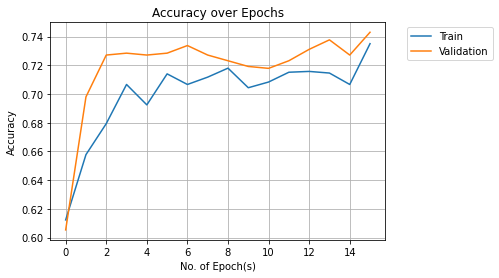
\includegraphics[width=0.5\textwidth]{accuracy-1.png}
	\caption{FastText Preprocessor - CNN Accuracy}
	\label{fig:ft-acc}
\end{figure}

\begin{figure}[h!]
	\centering
	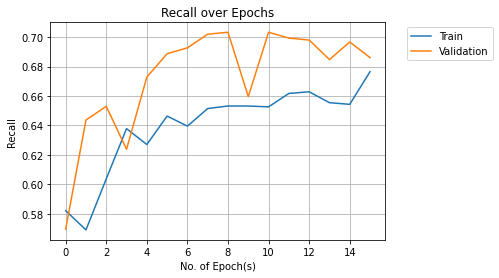
\includegraphics[width=0.5\textwidth]{recall-1.png}
	\caption{FastText Preprocessor - CNN Recall}
	\label{fig:ft-rec}
\end{figure}

For the second implementation, we observed that in \ref{fig:ft-acc} and
\ref{fig:ft-rec}, the validation accuracy and
recall was greater than that of training accuracy. We believe this can be
attributed to the regularization we used in the model to avoid overfitting,
which includes the four dropout layers that we added. This means that the model
at validation is more general and robust, which would in turn lead to a greater
validation accuracy and recall than training.

At the first epoch, the accuracy for the validation and training data are both
approximately 0.62, while recall is 0.57 and 0.58 respectively. The accuracy
for validation then rose and hovered around 0.73, while trraining oscilated
around 0.71. In regards to recall, the validation data experienced sudden drops
at the third and ninth epochs, but otherwise rose to about 0.7, while the
training data hovered around 0.65. Let us observe the models capacity to classify
our own written descriptions in \ref{fig:ft-con}.

\begin{figure}[h!]o
	\centering
	\includegraphics[width=0.5\textwidth]{confusion_matrix_ft.png}
	\caption{FastText Preprocessor - CNN Confusion Matrix}
	\label{fig:ft-con}
\end{figure}

In \ref{fig:ft-con}, we see that the model was fairly effective at classifying
depression, which had a precision and recall of 0.8, but struggled to accurately
label migraines and tetanus. When classifying migraines, the model had a
precision of 0.56 and recall of 1, however tetanus had a precision and recall of
0.

\subsection{Discussion}

\begin{figure}[h!]
	\centering
	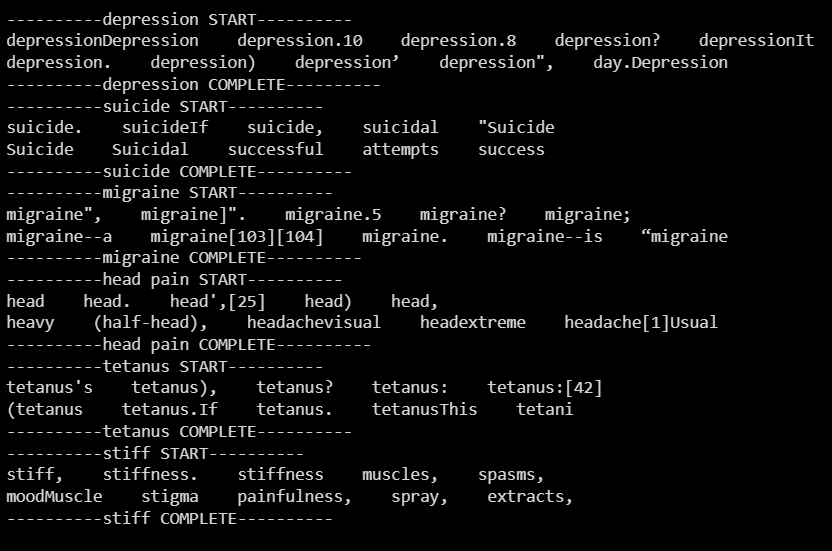
\includegraphics[width=0.5\textwidth]{proximate-words.png}
	\caption{The 10 most proximate words for depression, suicide, tetanus, stiff, migraine, head pain (in order).}
	\label{fig:prox-words}
\end{figure}

The intent behind the use of the FastText model primarly lied in
a belief, the retention of semantic meaning would allow the
model to connect terminology from the general domain to
terminology fom the medical domain. While there was some preliminary
indication that similar words were in close proximity, most words
only differed in punctuation as seen in Figure \ref{fig:prox-words}.
Simply put, the semantic meaning of each sentence was likely lost
during processing.

Furthermore, some sentences contained largely irrelevent bodies, such as
citations or questionaires. Thus, the dataset was diluted with elements that
potentially strayed the CNN from making correct classifications. This can be
seen in the model's inability to correctly classify custom Tetanus sentences,
where a majority of the citations where found. In retrospective, the drop
in accuracy could have been prevented through stricter filtering of the data
prior to feeding it to FastText model.


\chapter{Conclusion}

Through our examinations, we have tested the efficacy of a Convolutional Neural
Network's ability to classify descriptions of symptoms of an ailment as their
most probable diagnoses. In so doing, we created two implementations of a CNN,
one of which utilized generated training instances and One Hot Encoding while
the other used sentences from the corpus and word embeddings. Through testing
the two models ability to classify our written accounts of symptoms, we found
that the first implementation was more effective at accurately labelling
descriptions than the second. Going forward, there are several ways in which the
model can become more robust. The addition of more ailments and associated web
pages would provide more variety in the possible classifications the model can
discern.

\bibliography{report}

\end{document}
